
\chapter{UAV Topologies, standards and Communication Protocols}
\section*{Introduction}



In recent years, Unmanned Aerial Vehicles (UAVs) have evolved from specialized military tools into versatile platforms used in a wide range of civilian and commercial applications. This rapid development has resulted in a variety of UAV types, each designed for specific missions and operational needs. To better understand the technological landscape of UAVs, it is essential to examine their structural configurations, classification methods, and communication systems. This chapter presents an overview of UAV architectures from both design and performance perspectives. It also explores the key standards and communication protocols that enable their operation. The objective is to provide a clear picture of the current technological state of UAVs and their potential for integration into advanced systems.


%\subsection{History of Drones} 
\section{UAV Classification}


%%%%%%%%%%%%%%%%%%%%%%%%%%%%%%%%%%%%%%%%%%%%%%%%%%%%%%%%%%%%%%%%%%%%%%
%%%%%%%%%%%%%%%%%%%%%%%%%%%%%%%%%%%%%%%%%%%%%%%%%%%%%%%%%%%%%%%%%%%%%%
%%%%%%%%%%%%%%%%%%%%%%%%%%%%%%%%%%%%%%%%%%%%%%%%%%%%%%%%%%%%%%%%%%%%%%


Unmanned Aerial Vehicles (UAVs) have recently exhibited significant diversity in terms of design, functionality, and mission-specific adaptability. As their use expands across both civilian and military sectors, a robust classification framework becomes essential for understanding and optimizing their deployment. UAVs can be broadly categorized based on two major axes: \textbf{performance metrics} and \textbf{design architectures}.

\vspace{0.5cm}

\textit{Performance-based classification} involves measurable operational characteristics such as \textit{weight}, \textit{endurance}, \textit{range}, \textit{speed}, \textit{altitude}, \textit{wing loading}, and \textit{engine type}. These parameters are critical in determining how well a UAV meets specific mission requirements, such as long-range reconnaissance or high-speed target tracking.

\vspace{0.5cm}

In contrast, \textit{design-based classification} provides a structural perspective, focusing on aspects such as the \textit{aerodynamic configuration}, the \textit{number and arrangement of rotors or motors}, and the overall \textit{geometrical form}. This classification helps in understanding the UAV's flight behavior, stability, payload capacity, and maneuverability in various environments.


\begin{figure}[H]  % 'h' means place the figure "here" if possible
    \centering
    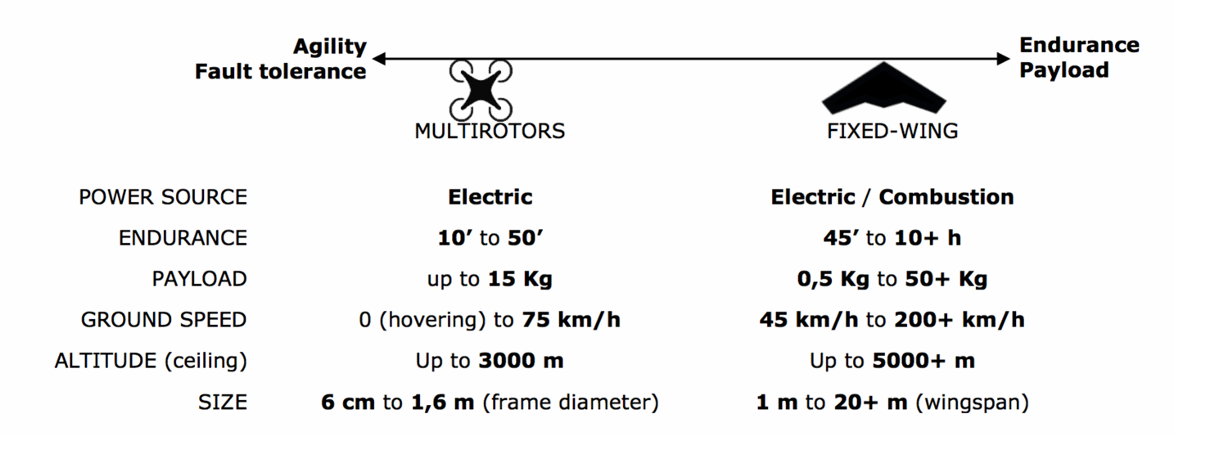
\includegraphics[width=0.7\textwidth]{Figures/Chapter1/Section1/1.png} % Adjust width as needed
    \caption{ Capabilities of fixed-wing/multi-rotors (adapted from: \cite{khan2024smarttraffic})}
    \label{fig:method3_architecture} % Reference label
\end{figure}


%%%%%%%%%%%%%%%%%%%%%%%%%%%%%%%%%%%%%%%%%%%%%%%%%%%%%%%%%%%%%%%%%%%%%%


\subsection{Design-Based Classification}

Design architecture plays a pivotal role in UAV functionality. UAVs can be structurally categorized into the following primary types. Figure~\ref{fig:uav_design_types} provides an overview of the primary UAV types based on design architecture.

\begin{figure}[H]  % 'h' means place the figure "here" if possible
    \centering
    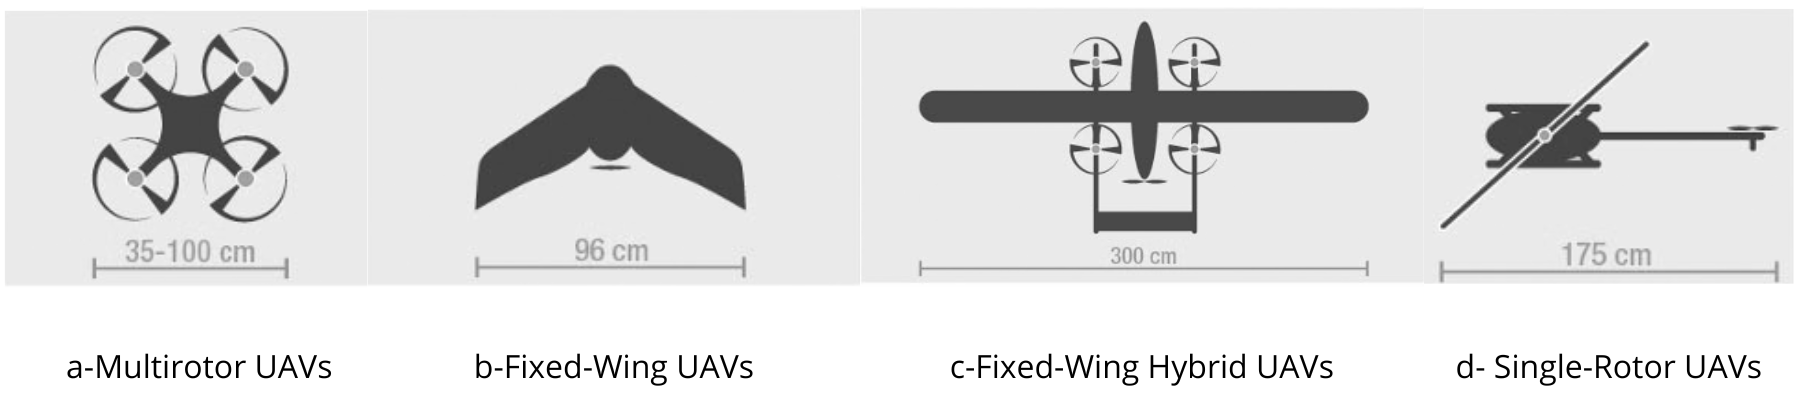
\includegraphics[width=0.7\textwidth]{Figures/Chapter1/Section1/11.png} % Adjust width as needed
    \caption{ Illustration of UAV Types Classified by Design )}
    \label{fig:uav_design_types}
\end{figure}


\begin{itemize}
    \item \textbf{Multirotor UAVs:} This category includes the most common drones used in commercial and consumer applications, featuring multiple rotors that allow for vertical lift, precise control, and stable hovering. Multirotor UAVs are typically employed in aerial photography, inspection, and surveillance tasks. The main types of multirotors are as follows:

    \begin{figure}[H]  % 'h' means place the figure "here" if possible
        \centering
        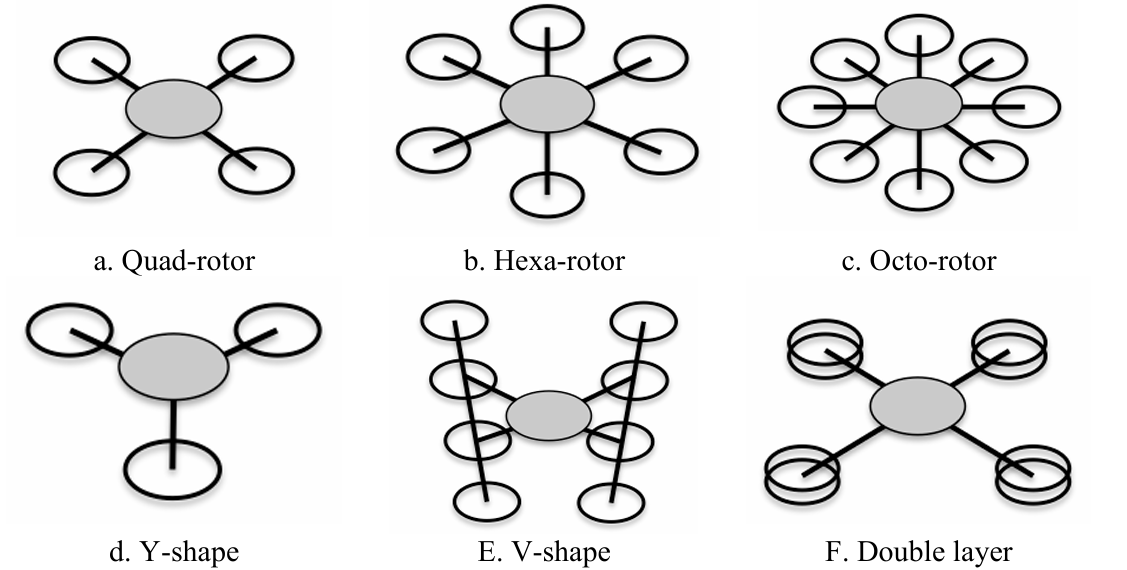
\includegraphics[width=0.7\textwidth]{Figures/Chapter1/Section1/2.png} % Adjust width as needed
        \caption{  Multi-rotors Layout  (adapted from: \cite{chen2016state})}
        \label{fig:method3_architecture} % Reference label
    \end{figure}
    
\begin{itemize}
    \item \textbf{Quad-rotor (4 Rotors):} Most common and cost-effective, offering stability for light-to-medium payloads. Limited redundancy single motor failure can destabilize flight. \cite{idk}
    
    \item \textbf{Hexa-rotor (6 Rotors):} Improved redundancy and payload capacity over quadcopters. Can tolerate one rotor failure but consumes more power. \cite{idk}
    
    \item \textbf{Octo-rotor (8 Rotors):} Highest redundancy and payload capacity, suited for critical missions. Sacrifices flight time due to high power demand. \cite{idk}
    
    \item \textbf{Y-shape Layout:} Three-rotor design for space efficiency. Lower redundancy and stability compared to quad/hexa configurations. \cite{idk}
    
    \item \textbf{V-shape Layout:} Aerodynamic efficiency for longer flight times. Compromises redundancy and stability. \cite{idk}
    
    \item \textbf{Double Layer Configuration:} Stacked rotors enhance lift in compact designs. Increases complexity and power usage. \cite{idk}
\end{itemize}
    
    \item \textbf{Fixed-Wing UAVs:} Fixed-wing UAVs generate lift via rigid wings, offering high efficiency for long-distance missions like mapping and surveying \cite{ucgun2021uavcharging}. They excel in speed and endurance but require runways for takeoff/landing, lacking VTOL capabilities. Compared to multirotors, they cover larger areas faster, making them ideal for large-scale data collection. Typical applications include military, agricultural, and scientific operations requiring extended flight times and higher payloads.

    % \begin{figure}[H]  % 'h' means place the figure "here" if possible
    %     \centering
    %     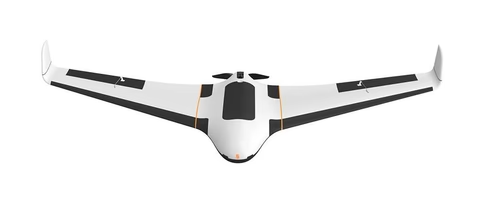
\includegraphics[width=0.7\textwidth]{Figures/Chapter1/Section1/3.png} 
    %     \caption{  Fixed-Wing UAVs (adapted from: site web uavsystemsinternational.com)}
    %     \label{fig:method3_architecture} % Reference label
    % \end{figure}

    \item \textbf{Fixed-Wing Hybrid UAVs:} Fixed-wing hybrid UAVs merge fixed-wing efficiency with rotary-wing VTOL capabilities, enabling flexible operation without runways. Their dual design allows long-range flight and quick deployment in confined spaces, ideal for search-and-rescue or surveillance. However, they are more complex and heavier than pure fixed-wing or multirotor UAVs.

    \item \textbf{Single-Rotor UAVs:} Single-rotor UAVs, like helicopters, use a main rotor for lift and a tail rotor for stability. They are more energy-efficient than multirotors, especially for heavy payloads, but have higher complexity and maintenance costs. Their advantages include longer flight times, better wind resistance, and suitability for cargo transport, surveying, and industrial inspections.
    
\end{itemize}

This classification provides a clear understanding of the different UAV types and their specific use cases based on design. Whether the goal is to achieve high endurance, heavy payload capabilities, or versatility in flight control, selecting the appropriate UAV design is essential for optimizing performance in various applications.



%%%%%%%%%%%%%%%%%%%%%%%%%%%%%%%%%%%%%%%%%%%%%%%%%%%%%%%%%%%%%%%%%%%%%%


\subsection{Performance-Based Classification}

Complementing the structural design perspective, UAVs can also be evaluated based on core operational parameters:

\begin{enumerate}
    \item \textbf{Weight:} Influences lift requirements, battery life, and legal classifications.

    UAVs span a wide spectrum of weights from micro UAVs under 5 kg to large strategic drones like the \textit{Global Hawk}, which exceeds 11 tonnes. Based on their take-off weight, UAVs can be classified into five categories:

    % \begin{itemize}
    %     \item \textbf{Micro UAVs (MAV):} Under 5 kg. Examples include the Dragon Eye, FPASS, Pointer, and SilentEyes.
    %     \item \textbf{Lightweight UAVs:} Between 5 kg and 50 kg.
    %     \item \textbf{Medium UAVs:} From 50 kg to 200 kg, such as the Raven up to the Phoenix.
    %     \item \textbf{Heavy UAVs:} Between 200 kg and 2000 kg, covering platforms like the Outrider to the Fire Scout.
    %     \item \textbf{Super Heavy UAVs:} Over 2 tonnes. This includes high-performance UAVs like the X-45, Predator B, Darkstar, and Global Hawk.
    % \end{itemize}

    \begin{table}[h]
        \centering
        \label{tab:uav_weights}
        \begin{tabular}{|l|l|l|}
        \hline
        \textbf{Category} & \textbf{Weight Range} & \textbf{Examples} \\ \hline
        Micro UAVs (MAV) & <5 kg & Dragon Eye, FPASS, Pointer \\ \hline
        Lightweight UAVs & 5-50 kg & - \\ \hline
        Medium UAVs & 50-200 kg & Raven, Phoenix \\ \hline
        Heavy UAVs & 200-2000 kg & Outrider, Fire Scout \\ \hline
        Super Heavy UAVs & >2000 kg & Global Hawk, X-45, Predator B \\ \hline
        \end{tabular}
        \caption{UAV Weight Classifications and Implications}
    \end{table}

    These categories influence design decisions across multiple domains: \textit{heavier UAVs require greater lift and thrust}, often leading to increased wingspan and a shift in engine technology (e.g., electric motors for light UAVs, turbojets or turbofans for super heavy ones).

    \item \textbf{Endurance and Range:} Critical for determining the mission duration and operational area.

    Endurance and range are often interdependent and essential for mission planning, especially in military and surveillance operations. UAVs can be grouped based on their time aloft:


    \begin{table}[h]
        \centering
        \label{tab:uav_endurance}
        \begin{tabular}{|l|l|l|}
        \hline
        \textbf{Category} & \textbf{Duration} & \textbf{Examples} \\ \hline
        Short Endurance & <5 hours & "Over-the-hill" reconnaissance UAVs \\ \hline
        Medium Endurance & 5-24 hours & Shadow 600, Predator \\ \hline
        Long Endurance & $\geq$24 hours & Global Hawk (1500-22000 km range) \\ \hline
        \end{tabular}
        \caption{UAV Endurance Classifications}
    \end{table}


    
    % \begin{itemize}
    %     \item \textbf{Short Endurance:} Less than 5 hours. Typically used for brief tactical missions like "over-the-hill" reconnaissance.
    %     \item \textbf{Medium Endurance:} Between 5 and 24 hours. Includes UAVs like the Shadow 600 and Predator this is the most common endurance class.
    %     \item \textbf{Long Endurance:} 24 hours or more. These UAVs are capable of extended surveillance with ranges starting at 1500 km and reaching up to 22000 km, as demonstrated by the Global Hawk.
    % \end{itemize}

    These parameters directly impact logistical planning, including launch site placement and refueling intervals.

    \item \textbf{Maximum Altitude:} Defines the UAV’s vertical operational limit, often constrained by regulatory frameworks.

    Maximum flight ceiling is critical in both civilian airspace integration and military stealth operations. UAVs are divided into:


    \begin{table}[h]
        \centering
        \label{tab:uav_altitude}
        \begin{tabular}{|l|l|l|}
        \hline
        \textbf{Category} & \textbf{Altitude Range} & \textbf{Examples} \\ \hline
        Low Altitude & Below 1,000 m & FPASS, Pointer, Dragon Eye \\ \hline
        Medium Altitude & 1,000-10,000 m & (Most common UAVs) \\ \hline
        High Altitude & Above 10,000 m & X-45, Predator B, Global Hawk \\ \hline
        \end{tabular}
        \caption{UAV Altitude Classifications}
    \end{table}



    % \begin{itemize}
    %     \item \textbf{Low Altitude:} Below 1000 meters. Examples include micro UAVs like the FPASS, Pointer, and Dragon Eye. These are mostly experimental or limited in use.
    %     \item \textbf{Medium Altitude:} Between 1000 m and 10000 m. The majority of UAVs fall into this category.
    %     \item \textbf{High Altitude:} Above 10000 m. This includes advanced UAVs like the X-45, Predator B, Darkstar, and Global Hawk. Operating at this altitude raises airspace integration concerns, necessitating advanced collision avoidance systems.
    % \end{itemize}

    \item \textbf{Wing Loading:} Affects aerodynamic performance, especially in varying weather conditions.

    Wing loading is defined as the UAV's weight divided by its wing area. It influences flight stability, speed, and maneuverability:

    \begin{table}[h]
        \centering
        \label{tab:uav_propulsion}
        \begin{tabular}{|l|l|l|}
        \hline
        \textbf{Propulsion} & \textbf{Application} & \textbf{Advantages} \\ \hline
        Electric & <50 kg UAVs & Zero emissions, simple control \\ \hline
        Piston & 50-2000 kg UAVs & Fuel flexibility, proven reliability \\ \hline
        Turbofan/Turbojet & >2000 kg UAVs & Supersonic capability, high altitude \\ \hline
        Turboprop & 500-5000 kg UAVs & Efficient cruise performance \\ \hline
        \end{tabular}
        \caption{UAV Propulsion Systems by Performance Characteristics}
    \end{table}

    High wing loading tends to enhance performance in strong winds but may reduce lift efficiency at lower speeds.

    \item \textbf{Engine Type:} Determines propulsion efficiency, noise levels, and maintenance needs.

    UAV engines vary widely based on mission needs. Common engine types include:

    \begin{table}[h]
        \centering
        \label{tab:uav_propulsion}
        \begin{tabular}{|l|l|l|}
        \hline
        \textbf{Propulsion} & \textbf{Application} & \textbf{Advantages} \\ \hline
        Electric & <50 kg UAVs & Zero emissions, simple control \\ \hline
        Piston & 50-2000 kg UAVs & Fuel flexibility, proven reliability \\ \hline
        Turbofan/Turbojet & >2000 kg UAVs & Supersonic capability, high altitude \\ \hline
        Turboprop & 500-5000 kg UAVs & Efficient cruise performance \\ \hline
        \end{tabular}
        \caption{UAV Propulsion Systems by Performance Characteristics}
    \end{table}

    \textit{Engine type is often interrelated with weight, endurance, and range.} Proper selection can significantly improve mission performance and energy efficiency.

    % \item \textbf{Power/Thrust Loading:} Indicates the UAV's ability to accelerate and maintain flight under load.

    This ratio reflects how efficiently a UAV can generate thrust relative to its weight. High thrust loading implies better climb rates and maneuverability, crucial in tactical and high-speed operations. Conversely, low thrust loading may indicate endurance-focused platforms optimized for loitering rather than agility.
\end{enumerate}

UAV performance depends on weight, endurance, altitude, wing loading, and propulsion. These factors determine mission capabilities, from short-range electric drones to long-endurance turbine-powered systems. Each design choice involves trade-offs between speed, stability, and efficiency.

%%%%%%%%%%%%%%%%%%%%%%%%%%%%%%%%%%%%%%%%%%%%%%%%%%%%%%%%%%%%%%%%%%%%%%


\subsection{Discussion}

The two classification approaches design-based  and performance-based offer complementary perspectives for UAV analysis. Design determines fundamental capabilities, while performance metrics define operational limits. Hybrid designs bridge gaps but introduce trade-offs in complexity.

\vspace{0.5cm}

Design dictates how a UAV flies, while performance defines how well it executes missions. Together, they form a framework for selecting UAVs tailored to specific applications, balancing structural advantages with operational requirements.

\subsubsection{}


%%%%%%%%%%%%%%%%%%%%%%%%%%%%%%%%%%%%%%%%%%%%%%%%%%%%%%%%%%%%%%%%%%%%%%
%%%%%%%%%%%%%%%%%%%%%%%%%%%%%%%%%%%%%%%%%%%%%%%%%%%%%%%%%%%%%%%%%%%%%%
%%%%%%%%%%%%%%%%%%%%%%%%%%%%%%%%%%%%%%%%%%%%%%%%%%%%%%%%%%%%%%%%%%%%%%


\section{UAV Characteristics}

Unmanned Aerial Vehicles (UAVs) come in a variety of configurations and are designed for different purposes, including surveillance, reconnaissance, and commercial applications. The performance of a UAV depends on several characteristics such as speed, flight time, payload capacity, range, and altitude. These parameters play a crucial role in determining the UAV's efficiency, mission capability, and operational limits. This section discusses the key characteristics of UAVs, providing an overview of the factors that influence their behavior and utility.


%%%%%%%%%%%%%%%%%%%%%%%%%%%%%%%%%%%%%%%%%%%%%%%%%%%%%%%%%%%%%%%%%%%%%%


\subsection{Speed and Flight Time}

The speed and flight time of UAVs are critical factors that determine their performance during operations. Smaller UAVs typically have a lower maximum speed, often less than 15 m/s, while larger UAVs can reach speeds up to 100 m/s. Speed plays an essential role in optimizing the energy consumption of UAVs, especially when following a specific trajectory designed for spectral or energy efficiency. As discussed in \cite{ref52}, there is a trade-off between a UAV's turning agility and its speed, which should be considered when planning flight paths.

\vspace{0.5cm}

Flight time, on the other hand, refers to the maximum duration a UAV can remain airborne before its battery is drained. Factors such as the UAV's size, weight, and external weather conditions significantly affect battery life. Larger UAVs generally have the capability to fly for several hours, while smaller UAVs may only remain in the air for 20–30 minutes. The autopilot system and GPS functionality can also influence flight time. With the growing demand for UAVs in various industries, improving their flight time is essential. Thus, ongoing research focuses on overcoming the limitations of battery life, which is crucial for the wide-scale deployment of UAVs in both military and commercial sectors.


%%%%%%%%%%%%%%%%%%%%%%%%%%%%%%%%%%%%%%%%%%%%%%%%%%%%%%%%%%%%%%%%%%%%%%


\subsection{Payload}

The payload capacity of a UAV refers to its ability to carry various loads, such as sensors, cameras, and other equipment. Payloads typically range from a few grams to hundreds of kilograms, depending on the UAV's size and design. The payload directly impacts the UAV's performance, as carrying heavier loads generally reduces its flight time, increases battery consumption, and requires a larger frame. For instance, UAVs often carry sensors and video cameras for surveillance, reconnaissance, or commercial purposes.

\vspace{0.5cm}

Additionally, UAVs can transport cellular user equipment (UE), such as mobile phones or tablets, with a weight of less than 1 kg. It is important to note that while heavier payloads can reduce flight time, UAVs with larger surface areas and additional motors can store more power, potentially extending flight duration. Therefore, the design of the UAV and the quality of the payload play a crucial role in determining its operational efficiency and endurance.


%%%%%%%%%%%%%%%%%%%%%%%%%%%%%%%%%%%%%%%%%%%%%%%%%%%%%%%%%%%%%%%%%%%%%%


\subsection{Range and Altitude}

The range and altitude of a UAV are key performance indicators that affect its operational capabilities. Range refers to the distance over which a UAV can be controlled remotely, varying from just a few meters for small drones to several hundred kilometers for larger UAVs. Altitude, on the other hand, defines the maximum height a UAV can achieve during flight. UAVs are typically categorized based on their operating altitude into two primary categories: low altitude platforms (LAPs) and high altitude platforms (HAPs).

\vspace{0.5cm}

\textbf{Low Altitude Platforms (LAPs):} LAPs are designed to support cellular communication systems and are typically deployed for quick and cost-effective operations. They offer line-of-sight (LoS) paths, which significantly enhance communication performance \cite{ref54}. These platforms are ideal for short-range missions and are often used in urban environments or areas with limited infrastructure.

\vspace{0.5cm}

\textbf{High Altitude Platforms (HAPs):} In contrast, HAPs, such as balloons, provide broader coverage and are used for more extensive communication or Internet connectivity services. The deployment of HAPs is more complex and generally requires advanced technology and infrastructure. While HAPs are capable of covering vast areas, they are typically utilized in more specialized applications, including large-scale communications or satellite-like coverage.

\vspace{0.5cm}

% Table \ref{tab:uav_categories} and Figure \ref{fig:uav_projects} further illustrate the differences between UAV types based on their altitude and operational range.


%%%%%%%%%%%%%%%%%%%%%%%%%%%%%%%%%%%%%%%%%%%%%%%%%%%%%%%%%%%%%%%%%%%%%%


\subsection{UAV Principal Movements}

UAVs rely on specific movements to navigate and perform tasks effectively. These movements are influenced by the design of the UAV and its control systems. The principal movements of UAVs can be broadly categorized as follows:

\vspace{0.5cm}

\textbf{1. Pitch:} The pitch movement refers to the rotation of the UAV around its lateral axis, which runs from one side of the aircraft to the other. A positive pitch angle results in the UAV's nose rising, while a negative pitch angle causes the nose to descend. This movement is crucial for controlling the altitude and vertical trajectory of the UAV.

\vspace{0.5cm}

\textbf{2. Roll:} Roll is the rotation of the UAV around its longitudinal axis, which runs from the nose to the tail of the aircraft. When the UAV rolls, one wing moves upward while the other moves downward, allowing the UAV to bank and change direction. Roll is essential for maintaining stability and adjusting the UAV's course during flight.

\vspace{0.5cm}

\textbf{3. Yaw:} Yaw refers to the rotation of the UAV around its vertical axis, which runs perpendicular to both the pitch and roll axes. A positive yaw rotates the UAV to the right, while a negative yaw rotates it to the left. Yaw is primarily responsible for controlling the UAV's heading and orientation.

% \textbf{4. Climb:} Climbing refers to the upward movement of the UAV, which is controlled by adjusting the pitch angle and increasing the thrust. This movement allows the UAV to gain altitude and is essential for reaching the desired flight height.

% \textbf{5. Descent:} Descent involves the downward movement of the UAV, often achieved by decreasing thrust and adjusting the pitch angle. This movement is necessary when the UAV needs to lower its altitude or land.

% \textbf{6. Hovering:} Hovering is the ability of a UAV to maintain a stationary position in the air. This is achieved by making fine adjustments to pitch, roll, yaw, and thrust. UAVs capable of hovering are particularly useful for tasks like aerial surveillance or photography, where precise positioning is crucial.

    \begin{figure}[H]  % 'h' means place the figure "here" if possible
        \centering
        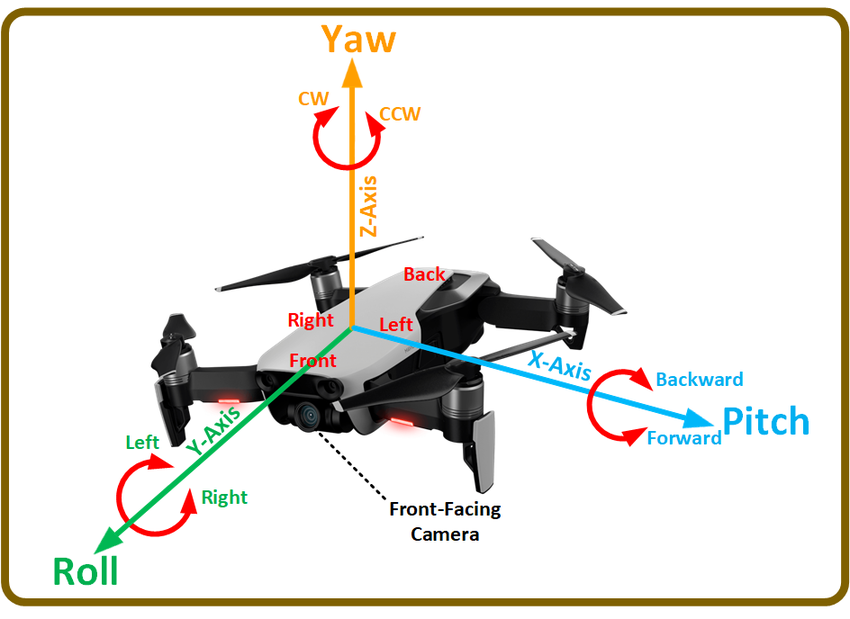
\includegraphics[width=0.7\textwidth]{Figures/Chapter1/Section2/1.png} 
        \caption{  Principal Movements of a UAV in 3D Space (adapted from: \cite{almahamid2024viznav})}
        \label{fig:method3_architecture} % Reference label
    \end{figure}


% These movements are essential for UAVs to navigate through their environment, maintain stability, and complete missions effectively. The ability to control these movements accurately is vital for ensuring the success of UAV operations, especially in dynamic and complex environments.

\vspace{0.5cm}

The characteristics of UAVs-such as speed, flight time, payload capacity, range, altitude, and principal movements are fundamental to their overall design and performance. Each characteristic impacts the UAV's ability to carry out specific tasks, whether it's surveillance, communication, or commercial applications. Understanding and optimizing these factors is essential for advancing UAV technology and ensuring the successful deployment of UAVs across various industries. As research continues to improve UAV designs, advancements in battery life, payload efficiency, and flight stability are expected to enhance the capabilities of UAVs, enabling them to perform more complex and longer-duration missions.


%%%%%%%%%%%%%%%%%%%%%%%%%%%%%%%%%%%%%%%%%%%%%%%%%%%%%%%%%%%%%%%%%%%%%%
%%%%%%%%%%%%%%%%%%%%%%%%%%%%%%%%%%%%%%%%%%%%%%%%%%%%%%%%%%%%%%%%%%%%%%
%%%%%%%%%%%%%%%%%%%%%%%%%%%%%%%%%%%%%%%%%%%%%%%%%%%%%%%%%%%%%%%%%%%%%%


\section{Communication protocols for UAVs}

Communication between the UAV and the Ground Control Station (GCS) relies on established communication protocols. However, existing protocols are not well-suited to the UAV environment. Due to the limited resources and the highly dynamic nature of unmanned systems, these protocols often fail to function efficiently according to \cite{larrieu2014model}.

\vspace{0.5cm}

This issue becomes even more critical when considering security measures, as UAVs typically operate with constraints such as limited battery life, restricted real-time processing power, and autonomous control requirements. Limited energy resources, communication bandwidth, and computational capacity make traditional protocols like TLS and Kerberos impractical for UAV networks.

\vspace{0.5cm}

Various communication protocols have been specifically developed for Unmanned Aerial Vehicles (UAVs). In this section, we will discuss these protocols in detail.


\subsection{UranusLink Protocol}


 UranusLink supports both unreliable and reliable packet‑oriented communication, defining the packet structure and the format in which data is transmitted. The protocol’s overall mechanism and detailed description are provided by Kriz et al.~\cite{kriz2015uranuslink}. In this study, we adopt their packet structure, as illustrated in Table~\ref{tab:uranuslink_pivoted}. Each packet comprises six fields: \textbf{Preamble} (PRE), \textbf{Sequence Number} (SQN), \textbf{Message Identification} (MID), \textbf{Data Length} (LEN), \textbf{Data}, and \textbf{Checksum} (CS).



\begin{table}[h]
\centering
\begin{tabular}{|c|c|c|c|c|c|c|}
\hline
\textbf{PRE} & \textbf{SQN} & \textbf{MID} & \textbf{LEN} & \textbf{DATA} & \textbf{CS} \\
\hline
1 B & 2 B & 1 B & 1 B & 1–252 B & 1 B \\
\hline
\end{tabular}
\caption{UranusLink packet structure. (adapted from \cite{kriz2015uranuslink})}
\label{tab:uranuslink_pivoted}
\end{table}

The UranusLink protocol is tailored for radio communications, where data loss and corruption are frequent.  Each packet begins with a \textbf{preamble (PRE)} byte \texttt{0xFD}, which seldom occurs in payloads, ensuring reliable packet boundary detection.  Following this is an even-valued \textbf{sequence number (SQN)}, used to detect lost or out of order packets any packet with an SQN lower than the last accepted is discarded and a \textbf{checksum (CS)} to validate integrity.  The sizes of PRE and CS balance robustness against overhead, taking link conditions and capacity into account.

\vspace{0.5cm}

The \textbf{MID} field specifies how to interpret the payload.  Currently there are eight UAV to ground and sixteen ground‑to‑UAV message types; the two critical ones establish and maintain the connection in each direction.  

\vspace{0.5cm}

Two UAV modes are supported: \textbf{flight mode}, in which the rotors spin, and \textbf{configuration mode}, used on the ground.  A “robot mode switch” message triggers transitions, and only these mode‑switch packets are acknowledged other messages are sent unacknowledged to minimize overhead.  The ground station tracks SQNs of mode switch requests so it can determine the UAV’s current mode even if acknowledgments are lost.

\vspace{0.5cm}

Compared to MAVLink which can incur up to 33 \% extra overhead and offers no built‑in security UranusLink achieves much lower overhead while providing essential reliability and mode‑switch acknowledgment.



\subsection{UAVCAN protocol}

UAVCAN is an open‑source, masterless publish–subscribe protocol for secure connectivity over CAN buses in aerospace and robotics.  It carries long payloads in a single CAN frame (e.g.\ GNSS fixes, 3D vectors), supports multiple nodes and interfaces for high‑safety applications, and offers standard services such as network discovery, node configuration and firmware upgrade, status monitoring, time synchronization, and adaptive node‑ID allocation.  Lightweight and real‑time–capable, UAVCAN is ideal for resource‑constrained UAVs and is released under the MIT license \cite{kriz2015uranuslink}.

\vspace{0.5cm}

Based on the CAN bus, originally created for automotive multiplex wiring, UAVCAN enables host‑free communication between devices and microcontrollers \cite{kriz2015uranuslink}.  Each node is assigned a unique ID in the range 1–127 (ID 1 typically denotes the autopilot; 126–127 are for debugging).  To avoid mismatches, any MAVLink component communicating over UAVCAN must use the same Component ID (COMPID) as its UAVCAN Node ID commonly both set to 1 so that every MAVLink message’s COMPID field matches its UAVCAN node ID \cite{kriz2015uranuslink}.




\subsection{MAVLink protocol}


MAVLink is an open and efficient communication protocol tailored for lightweight, real-time interactions between Unmanned Aerial Vehicles (UAVs) and Ground Control Stations (GCSs). Developed by Lorenz Meier and first released in 2009 under the LGPL license, MAVLink 1.0 quickly became popular thanks to its streamlined design and operational simplicity \cite{allouch2019mavsec, koubaa2017mavlink}. A significant evolution of the protocol occurred in 2017 with the introduction of MAVLink 2.0, which is currently the preferred version. It maintains backward compatibility with MAVLink 1.0 while offering improvements in extensibility, robustness, and security features.

\vspace{0.5cm}

MAVLink messages are broadly categorized into two types: those originating from the GCS to issue commands or control instructions to UAVs, and those transmitted by UAVs to the GCS, typically conveying telemetry data such as geographical coordinates, altitude, system heartbeat, and operational status. To meet the demands of real-time systems, MAVLink was designed with minimal communication overhead to ensure high efficiency \cite{allouch2019mavsec}. The following sections provide a comparative overview of the header structures used in MAVLink 1.0 and its successor, MAVLink 2.0.



\subsubsection{MAVLink 1.0 header protocol}


The comprehensive survey by Koubaa et al. \cite{koubaa2017mavlink} remains the only detailed study focused on the MAVLink protocol’s architecture and operational principles. As part of their contribution, the authors present the header structure for MAVLink 1.0. Below, we describe the structure of a MAVLink 1.0 frame, which consists of eight primary fields, as illustrated in Figure~\ref{fig:mavlink-v1-packet}.

The first byte, labeled \textbf{STX}, has a fixed value of \texttt{0xFE}, which identifies the start of a MAVLink 1.0 message frame. The second field, \textbf{LEN}, encoded in one byte, indicates the length of the payload. The third field, \textbf{SEQ}, is also one byte and stores a sequence number ranging from 0 to 255. Once 255 is reached, it rolls over to 0. This sequence number helps in detecting lost packets.

To distinguish between multiple UAVs managed by a single Ground Control Station, the fourth field, \textbf{SYS ID}, is used. This field also spans one byte, limiting the addressable systems to 254 UAVs, since ID 255 is typically reserved for the GCS. The fifth field, \textbf{COMP ID}, identifies the specific component (e.g., autopilot, gimbal) transmitting the message. Finally, the sixth byte marks the beginning of the payload section, which contains the message-specific data.

\begin{figure}[ht]
\centering
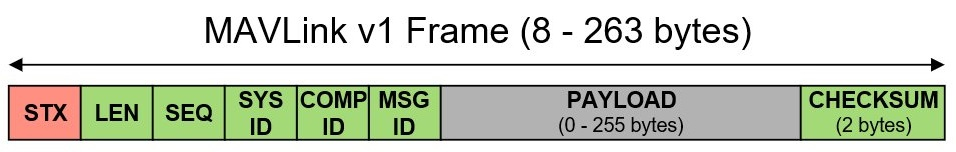
\includegraphics[width=0.9\textwidth]{Figures/Chapter1/Section4/1.jpg} % Save image locally
\caption{Structure of a MAVLink 1.0 packet \cite{mavlinkio}.}
\label{fig:mavlink-v1-packet}
\end{figure}





\begin{table}[ht]
\renewcommand{\arraystretch}{1.3} % Slightly more vertical space for centering
\centering
\caption{MAVLink 1.0 header structure and byte size. (adapted from \cite{koubaa2017mavlink})}
\begin{tabular}{|>{\centering\arraybackslash}m{2.5cm}|
                >{\centering\arraybackslash}m{2cm}|
                >{\arraybackslash}m{7cm}|}
\hline
\textbf{Field} & \textbf{Size} & \textbf{Description} \\
\hline
STX & 1 B & \vspace{0pt}Start-of-frame indicator (0xFE in MAVLink 1.0). \\
\hline
LEN & 1 B & \vspace{0pt}Payload length (0–255 bytes). \\
\hline
SEQ & 1 B & \vspace{0pt}Packet sequence number (0–255, wraps after 255). Used to detect packet loss. \\
\hline
SYS ID & 1 B & \vspace{0pt}System identifier (e.g., UAV ID). Value 255 is typically used by the GCS. \\
\hline
COMP ID & 1 B & \vspace{0pt}Component identifier (e.g., autopilot or camera module). \\
\hline
Message ID & 1 B & \vspace{0pt}Indicates the type of MAVLink message. \\
\hline
Payload & 0–255 B & \vspace{0pt}Actual message data depending on message type. \\
\hline
Checksum (CRC) & 2 B & \vspace{0pt}Verifies the integrity of the packet (LSB to MSB order). \\
\hline
\end{tabular}
\label{tab:mavlink_header}
\end{table}





In summary, the MAVLink 1.0 protocol employs a lightweight and efficient packet structure that balances low bandwidth usage with sufficient message integrity. The use of fixed-length headers, flexible payloads up to 255 bytes, and a robust CRC-based checksum mechanism ensures reliable communication between UAVs and ground stations. Understanding the role of each header field, especially the \texttt{Message ID}, is essential for correctly interpreting messages and extracting relevant data from the payload.



\subsubsection{MAVLink 2.0 Protocol}

MAVLink 2.0 was introduced in early 2017 \cite{allouch2019mavsec, khan2020emerging}, offering enhancements over MAVLink 1.0 while maintaining backward compatibility. This section presents the MAVLink 2.0 header structure and compares it with MAVLink 1.0. The MAVLink 2.0 header is shown in Fig.~\ref{fig:mavlink-v2-packet}, and Table~\ref{tab:mavlink2_additional_fields} explains the additional fields in the MAVLink 2.0 header compared to MAVLink 1.0.

\vspace{0.5cm}

MAVLink 2.0 retains all fields from MAVLink 1.0 but adds new fields and expands some existing ones. The first byte (0xFD) marks the start of the message, differing from MAVLink 1.0's 0xFE. The payload length field remains unchanged. Two flags appear before the sequence number (SEQ): the incompatibility flag, which indicates if the packet is signed, and the compatibility flag, which does not affect the message structure.

\begin{figure}[ht]
\centering
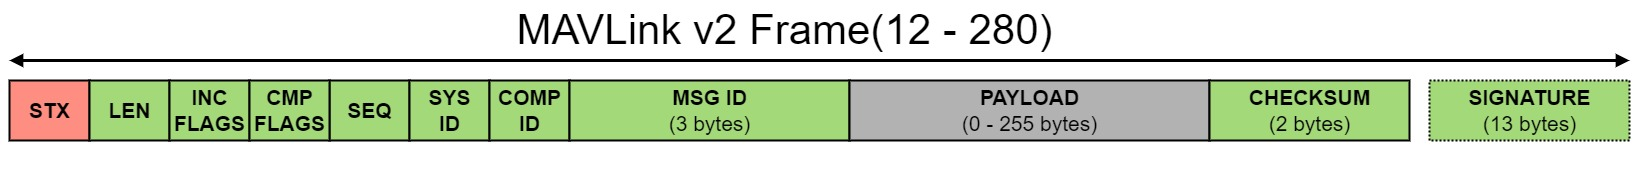
\includegraphics[width=0.8\textwidth]{Figures/Chapter1/Section4/2.jpg}
\caption{MAVLink 2.0 Header Structure.}
\label{fig:mavlink-v2-packet}
\end{figure}


\begin{table}[H]
\renewcommand{\arraystretch}{1.3} % Slightly more vertical space for centering
\centering
\caption{Additional MAVLink 2.0 Header Fields (compared to MAVLink 1.0).}
\begin{tabular}{|>{\centering\arraybackslash}m{2.5cm}|
                >{\centering\arraybackslash}m{2cm}|
                >{\arraybackslash}m{7cm}|}
\hline
\textbf{Field} & \textbf{Size} & \textbf{Description} \\
\hline
STX & 1 B & \vspace{0pt}Start-of-frame indicator (0xFD in MAVLink 2.0). \\
\hline
Incompatibility Flag & 1 B & \vspace{0pt}Indicates whether the message is signed (e.g., 0x01 indicates signed message). \\
\hline
Compatibility Flag & 1 B & \vspace{0pt}Indicates compatibility options that can be ignored by parsers if not recognized. \\
\hline
MSGID & 3 B & \vspace{0pt}Message identifier, expanded from 8 bits in MAVLink 1.0 to 24 bits in MAVLink 2.0, allowing up to 16,777,215 different message types. \\
\hline
Signature & 13 B & \vspace{0pt}Used for message authentication, ensuring integrity and authenticity, including LinkID, Timestamp, and the actual Signature field. \\
\hline
\end{tabular}
\label{tab:mavlink2_additional_fields}
\end{table}

The SEQ (sequence number), system ID, and COMPID fields in MAVLink 2.0 are identical to those in MAVLink 1.0. The MSGID field is expanded from 8 to 24 bits, increasing the number of possible messages to over 16 million. The payload field can carry up to 255 bytes. The checksum in MAVLink 2.0 remains the same as in MAVLink 1.0.

\vspace{0.5cm}

MAVLink 2.0 introduces a 13-byte field for message authentication, improving security over MAVLink 1.0. The message signature is appended when the incompatibility flag is set to 0x01. This addition significantly enhances security by ensuring message integrity and authenticity.

\vspace{0.5cm}

The 13-byte message signature contains the following fields:
\begin{itemize}
    \item \textbf{LinkID:} A one-byte field representing the link (channel) used to send the packet. The link refers to any telemetry device (e.g., Wi-Fi). Each channel used to send information has a unique LinkID.
    \item \textbf{Timestamp:} Encoded as 6 bytes in 10-microsecond units, the timestamp represents the time since January 1, 2015 GMT. The timestamp increases with each message sent over the channel and helps prevent replay attacks.
    \item \textbf{Signature:} This field covers the full message, the secret key, and the timestamp. It is encrypted into 6 bytes for the message. The first 6 bytes (48 bits) of a SHA-256 hash applied to the MAVLink 2.0 message are included in the signature. A 32-byte shared symmetric key is stored on both ends, i.e., the autopilot and the ground station or the MAVLink API.
\end{itemize}

Messages are discarded if: (1) they are received earlier than a previous packet from the same tuple (LinkID, SystemID, ComponentID); (2) the signature does not match; or (3) the timestamp exceeds one minute compared to the local system time \cite{koubaa2017mavlink}.




\subsection{ Disscussion}


UAV operations depend critically on communication protocols that remain vulnerable despite widespread use. Current protocols like MAVLink, UranusLink, and UAVCan (compared in Table~\ref{tab:uav_protocol_comparison}) each compromise between functionality, maturity, and crucial security features.




\begin{table}[H]
\centering
\renewcommand{\arraystretch}{1.0} % Reduced from 1.3
\setlist[itemize]{nosep,leftmargin=*,topsep=0pt,partopsep=0pt} % Compact lists
\begin{tabular}{|>{\centering\arraybackslash}m{3cm}|
                >{\arraybackslash}m{6cm}|
                >{\arraybackslash}m{6cm}|}
\hline
\textbf{Protocol} & \textbf{Pros} & \textbf{Limitations} \\ 
\hline
UranusLink & 
\begin{itemize}
    \item Open-source
    \item Lightweight
    \item Aerospace/robotic focus
    \item Redundant transports
\end{itemize} & 
\begin{itemize}
    % \item Unstable version
    \item Limited language support
    \item No concurrency
    \item Not scalable
    \item Lacks security
\end{itemize} \\ 
\hline
UAVCan & 
\begin{itemize}
    \item Open-source
    \item Lightweight
    \item Low latency
    \item Data loss recovery
\end{itemize} & 
\begin{itemize}
    \item Limited language support
    \item No concurrency
    \item Not scalable
\end{itemize} \\ 
\hline
MAVLink & 
\begin{itemize}
    \item Widely accepted
    \item Scalable
    \item Multi-language
    \item Concurrent systems
    \item Proven performance
\end{itemize} & 
\begin{itemize}
    \item No payload security
    \item Weak encryption
    \item Small data only
    \item Open format
\end{itemize} \\ 
\hline
\end{tabular}
\caption{Comparison of UAV Communication Protocols}
\label{tab:uav_protocol_comparison}
\end{table}





As evidenced in Table~\ref{tab:uav_protocol_comparison}, current UAV protocols prioritize lightweight operation and low latency at the expense of robust security - particularly MAVLink, whose widespread use in critical operations contrasts sharply with its lack of payload encryption and authentication \cite{khan2020emerging}. These security gaps create attack vectors for message spoofing, data interception, and even UAV hijacking, with potentially catastrophic consequences for sensitive operations ranging from military reconnaissance to emergency response missions. The protocol limitations underscore an urgent need for security-enhanced communication frameworks that maintain performance while addressing these vulnerabilities.






%%%%%%%%%%%%%%%%%%%%%%%%%%%%%%%%%%%%%%%%%%%%%%%%%%%%%%%%%%%%%%%%%%%%%%
%%%%%%%%%%%%%%%%%%%%%%%%%%%%%%%%%%%%%%%%%%%%%%%%%%%%%%%%%%%%%%%%%%%%%%
%%%%%%%%%%%%%%%%%%%%%%%%%%%%%%%%%%%%%%%%%%%%%%%%%%%%%%%%%%%%%%%%%%%%%%


\section{UAVs Architectures}



The communication architecture is essential for enabling intelligent control and autonomous collaboration in UAV swarms. Initially, centralized architectures an extension of traditional single-UAV systems were used, with a single ground station managing all UAV communication. However, as swarm size and mission complexity grew, decentralized architectures emerged as more scalable alternatives, reducing dependency on central nodes \cite{Cao2012}. Many studies have since explored different swarm communication models. This section reviews the main architectures, summarizing their characteristics, strengths, and limitations.




%%%%%%%%%%%%%%%%%%%%%%%%%%%%%%%%%%%%%%%%%%%%%%%%%%%%%%%%%%%%%%%%%%%%%%


\subsection{Centralized Communication Architecture}
\label{sec:centralized}

The \textbf{centralized communication architecture}, adapted from single-UAV systems, was later applied to UAV swarms. As shown in \textbf{Figure~\ref{fig:centralized communication architecture}}, it relies on a central node, such as fixed network infrastructure, connecting all UAVs through direct one-to-one links without intermediary relays. This setup offers routing simplicity, stability, and efficient performance at small scales. It is best suited for missions with limited swarm size, coverage, and complexity. A notable implementation is the \textbf{"UAV-GCS Centralized Data-Oriented Communication Architecture"} used in crowd surveillance \cite{Chen2020}.


\begin{figure}[H]
\centering
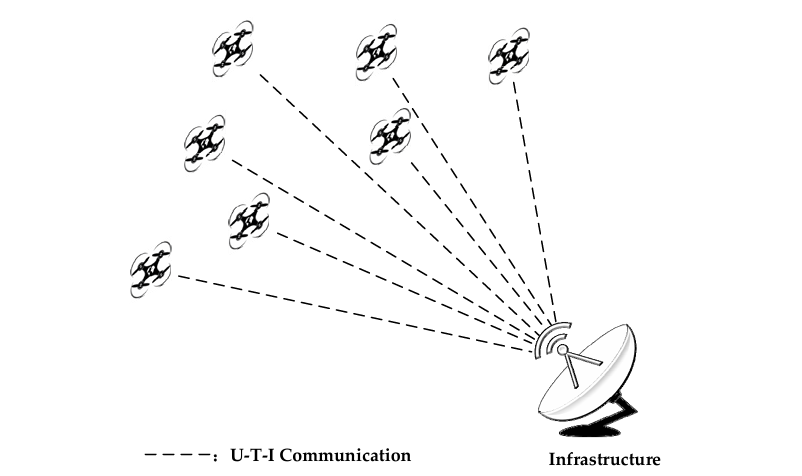
\includegraphics[width=0.8\textwidth]{Figures/Chapter1/Section5/1.png}
\caption{centralized communication architecture \cite{Chen2020}}
\label{fig:centralized communication architecture}
\end{figure}

Despite its simplicity, this architecture presents key limitations. All inter-UAV communication must pass through the infrastructure, making the \textbf{UAV-to-Infrastructure (U-T-I)} distance typically longer than the \textbf{UAV-to-UAV (U-T-U)} distance, resulting in increased latency. Moreover, the high mobility of UAVs and growing coverage requirements render the system unstable. A major weakness is its \textbf{Single Point of Failure (SPOF)} if the ground station or satellite fails, the entire network collapses. As a result, centralized architectures are unsuitable for large-scale or high-risk missions.



%%%%%%%%%%%%%%%%%%%%%%%%%%%%%%%%%%%%%%%%%%%%%%%%%%%%%%%%%%%%%%%%%%%%%%


\subsection{Decentralized Communication Architecture}

Given the high operational speeds of UAVs and the extensive coverage demands of missions, network connectivity often fluctuates as UAVs dynamically join and leave the network. This variability makes ad hoc networking ideal for UAV swarms. In decentralized architectures, UAVs establish real-time, self-organizing connections, eliminating the need for fixed infrastructure and overcoming traditional communication range limitations \cite{Chen2020}.



\subsubsection{Single-Group Swarm Ad Hoc Network}

In a single-group swarm ad hoc network (~\ref{fig:single-group_swarm_Ad_hoc_network}), communication occurs independently of fixed infrastructure, with a gateway UAV linking the swarm to external systems and other UAVs acting as relay nodes to distribute data. This structure supports real-time information sharing among swarm members, improving operational efficiency. The gateway UAV uses two transceivers: a short-range, low-power unit for intra-swarm communication and a long-range, high-power system for external links \cite{Chen2020}. This design enables the use of lightweight transceivers in regular UAVs, extending coverage and accommodating smaller UAVs. However, the system requires uniform flight patterns, making it well-suited for homogeneous small UAV groups. When applied to heterogeneous swarms with different UAV types, variations in operational characteristics prevent close formation flying, leading to the development of more adaptable multi-group and multi-layer architectures for complex mission needs.


\begin{figure}[ht]
\centering
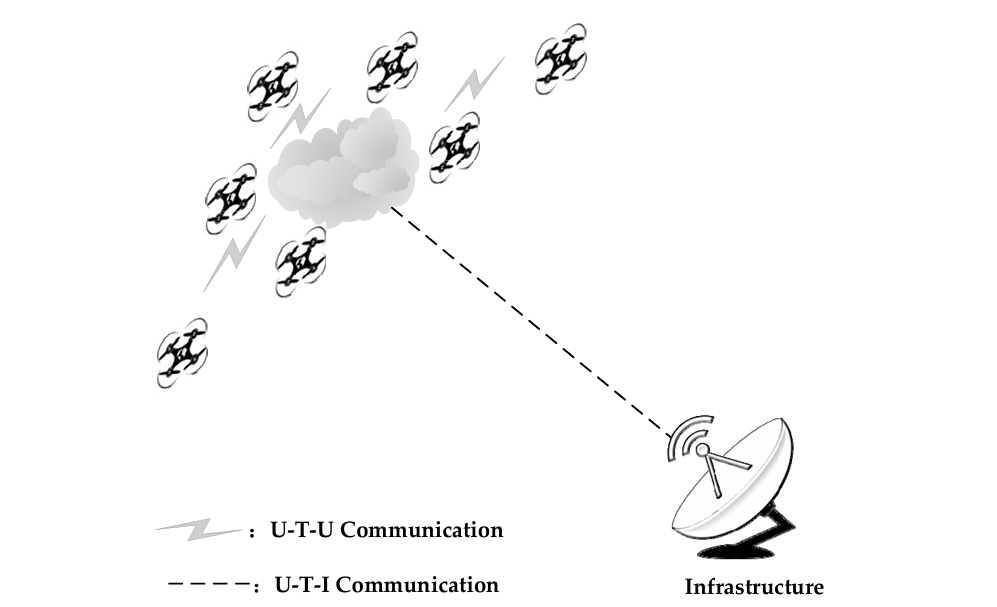
\includegraphics[width=0.8\textwidth]{Figures/Chapter1/Section5/2.png}
\caption{single-group swarm Ad hoc network \cite{Chen2020}}
\label{fig:single-group_swarm_Ad_hoc_network}
\end{figure}


% \vspace{0.5cm}

Several intra-swarm communication  configurations (~\ref{fig:intra-swarm communication architecture}) have emerged:
\begin{itemize}
\item \textbf{Ring Architecture}: Forms a closed communication loop where any UAV can serve as gateway, providing redundancy but limited scalability
\item \textbf{Star Architecture}: Centralizes communication through a gateway UAV, creating a single point of failure vulnerability
\item \textbf{Meshed Architecture}: Combines ring and star advantages, allowing any UAV to function as a gateway with multiple routing paths
\end{itemize}

While meshed architecture has become the standard for its flexibility, mission diversity increasingly requires swarms to incorporate varied UAV sizes and capabilities, pushing the development of more advanced network topologies.





\begin{figure}[ht]
\centering
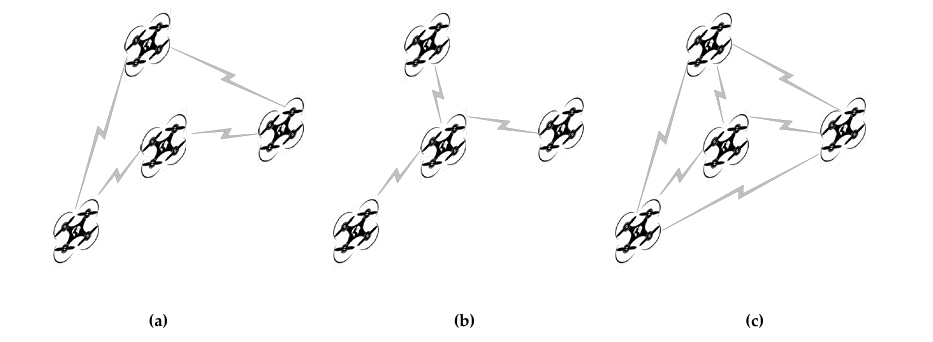
\includegraphics[width=0.7\textwidth]{Figures/Chapter1/Section5/3.png}
\caption{intra-swarm communication architecture: (a): ring rchitecture, (b) star architectue, (c): meshedarchitecture. \cite{Chen2020}}
\label{fig:intra-swarm communication architecture}
\end{figure}


\subsubsection{Multi-Group Swarm Ad hoc Network}

The \textit{multi-group swarm Ad hoc network} (Figure~\ref{fig:multi-group swarm Ad hoc network}) combines elements of both centralized and \textit{single-group swarm Ad hoc network} architectures to address the limitations of the latter. Each group, depending on its mission, operates in an Ad hoc manner for intra-group communication, while inter-group communication (Group-to-Group or G-T-G) relies on the infrastructure, with gateway UAVs handling communication with the central infrastructure. This architecture is semi-centralized, and while it can accommodate diverse UAV types for complex missions, it still suffers from high latency in G-T-G communications. The \textit{multi-group swarm Ad hoc network} is particularly suitable for applications like multi-theater joint operations in military scenarios, where a central control center coordinates UAV swarms that approach the mission area from various directions~\cite{kaleem2019uav}.


\begin{figure}[ht]
\centering
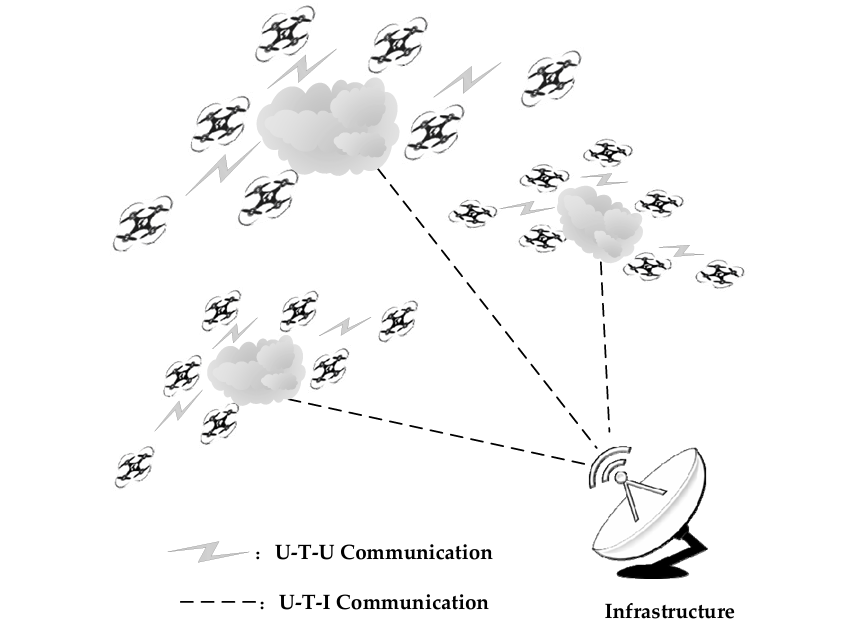
\includegraphics[width=0.6\textwidth]{Figures/Chapter1/Section5/4.png}
\caption{multi-group swarm Ad hoc network \cite{Chen2020}}
\label{fig:multi-group swarm Ad hoc network}
\end{figure}



\subsubsection{Multi-layer Swarm Ad hoc Network}


The \textit{multi-layer swarm Ad hoc network} architecture, as depicted in Figure~\ref{fig:multi-layer swarm Ad hoc network}, is a more advanced version of the \textit{multi-group swarm Ad hoc network}. In this architecture, UAVs of the same type form an Ad hoc network at the first layer, enabling intra-group communication. At the second layer, gateway UAVs facilitate Group-to-Group (G-T-G) communication between different UAV groups. The third layer consists of the gateway UAVs communicating with the infrastructure. Notably, UAVs in the same group can communicate directly without infrastructure relay, while inter-group communication passes through the gateway UAV \cite{Chen2020} Data packets move through the first and second layers sequentially, ensuring there is no single point of failure (SPOF). This multi-layer structure offers increased robustness compared to other architectures.


\begin{figure}[ht]
\centering
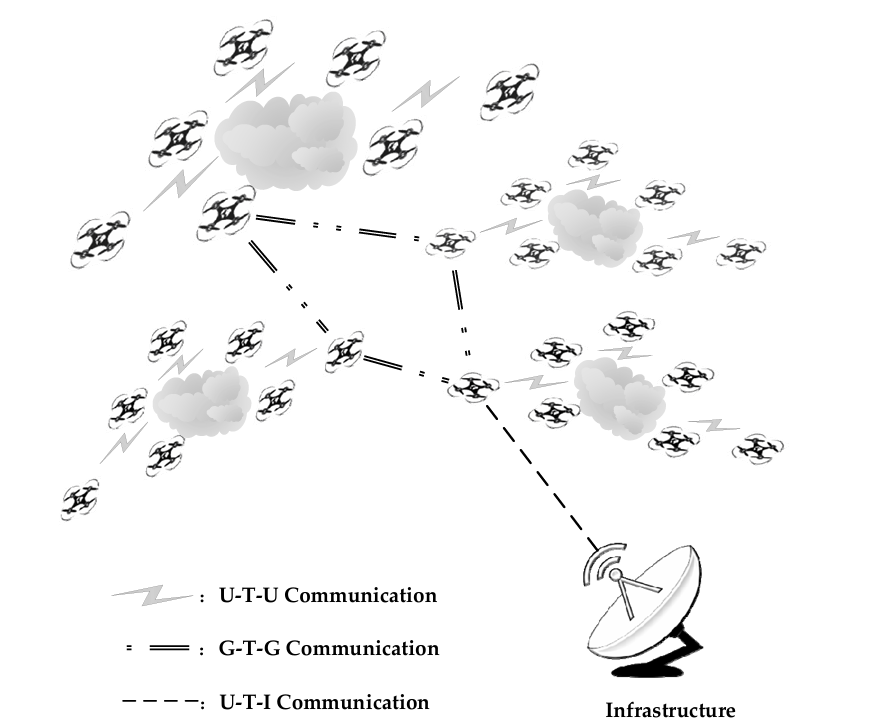
\includegraphics[width=0.6\textwidth]{Figures/Chapter1/Section5/5.png}
\caption{multi-layer swarm Ad hoc network \cite{Chen2020}}
\label{fig:multi-layer swarm Ad hoc network}
\end{figure}


The \textit{multi-layer swarm Ad hoc network} architecture adapts to changes in UAV numbers, enabling quick network reconstruction. It is ideal for complex missions with dynamic network topologies and frequent UAV communication. Future improvements may include adding more layers to enhance task coverage and network robustness.


%%%%%%%%%%%%%%%%%%%%%%%%%%%%%%%%%%%%%%%%%%%%%%%%%%%%%%%%%%%%%%%%%%%%%%


\subsection{Discussion}


UAV swarm communication architecture has advanced significantly, with various options for different mission scenarios. Centralized architecture suits small, simple missions with long-range communication to infrastructure \cite{Chen2020}. Decentralized architecture extends coverage via multi-hop networks and gateway UAVs for UAV-to-infrastructure communication. The \textit{single-group swarm Ad hoc network} works for homogenous UAVs, while the \textit{multi-group} and \textit{multi-layer swarm Ad hoc network} architectures are better for diverse UAV types, though the former may face delays in inter-group communication. The \textit{multi-layer swarm Ad hoc network} is more robust, eliminating single point of failure (SPOF).




\begin{table}[H]
\centering
\renewcommand{\arraystretch}{1.0}
\setlist[itemize]{nosep,leftmargin=*,topsep=0pt,partopsep=0pt}
\begin{tabular}{|>{\centering\arraybackslash}m{3.5cm}|
                >{\centering\arraybackslash}m{2.2cm}|
                >{\centering\arraybackslash}m{2.2cm}|
                >{\centering\arraybackslash}m{2.2cm}|
                >{\centering\arraybackslash}m{2.2cm}|
                >{\centering\arraybackslash}m{2.2cm}|}
\hline
\textbf{Features} & \textbf{Centralized} & \textbf{Decentralized} & \textbf{Single-Group} & \textbf{Multi-Group} & \textbf{Multi-Layer} \\
\hline
Multi-hop Communication & x & \checkmark & \checkmark & \checkmark & \checkmark \\
\hline
UAVs Relay Traffic      & x & \checkmark & \checkmark & \checkmark & \checkmark \\
\hline
Different Types of UAVs & x & \checkmark & x & \checkmark & \checkmark \\
\hline
Self-configuration      & x & \checkmark & \checkmark & \checkmark & \checkmark \\
\hline
Limited Coverage        & \checkmark & x & x & x & x \\
\hline
Single Point of Failure & \checkmark & x & x & x & x \\
\hline
Robustness              & x & \checkmark & \checkmark & \checkmark & \checkmark \\
\hline
\end{tabular}
\caption{Summary of UAV Swarm Communication Architectures (\checkmark = supported, x = not supported) \cite{Chen2020}}
\label{tab:swarm_architecture_summary}
\end{table}


UAV swarm communication architectures must balance high coverage and connectivity. Coverage is key for intelligence gathering, while connectivity ensures real-time communication. However, dynamic environments make maintaining connectivity challenging due to signal attenuation. To avoid disruption, UAVs must stay within a suitable distance for effective communication. Nature-inspired behaviors can improve positioning, and advancements in 4G and 5G networks offer potential solutions for better connectivity across wide areas.



%%%%%%%%%%%%%%%%%%%%%%%%%%%%%%%%%%%%%%%%%%%%%%%%%%%%%%%%%%%%%%%%%%%%%%
%%%%%%%%%%%%%%%%%%%%%%%%%%%%%%%%%%%%%%%%%%%%%%%%%%%%%%%%%%%%%%%%%%%%%%
%%%%%%%%%%%%%%%%%%%%%%%%%%%%%%%%%%%%%%%%%%%%%%%%%%%%%%%%%%%%%%%%%%%%%%


\section{Routing Protocols}


This section reviews common UAV swarm communication routing technologies, classifies routing protocols based on their underlying techniques, and provides a detailed overview of each category, highlighting their pros and cons. Building on prior comparisons of current architectures where the multi-layer swarm Ad hoc network showed the best overall performance it emphasizes the critical role of routing in ensuring reliable U-T-U communication, despite challenges like UAV mobility, unstable links, limited resources, and varying QoS needs. Traditional Ad hoc protocols require adaptation, making the design of suitable routing protocols a key research focus.


%%%%%%%%%%%%%%%%%%%%%%%%%%%%%%%%%%%%%%%%%%%%%%%%%%%%%%%%%%%%%%%%%%%%%%

\subsection{Routing Technologies}

Routing technologies form the foundation for implementing routing protocols, which are often built by enhancing or combining these basic techniques. Since UAV swarm Ad hoc networks evolve from traditional Ad hoc networks, conventional routing methods can still be applied after suitable analysis and adaptation. The six common routing technologies used include store-carry-forward, greedy forwarding, path discovery, single-path, multi-path, and predictive routing \cite{Chen2020}.


\begin{figure}[ht]
\centering
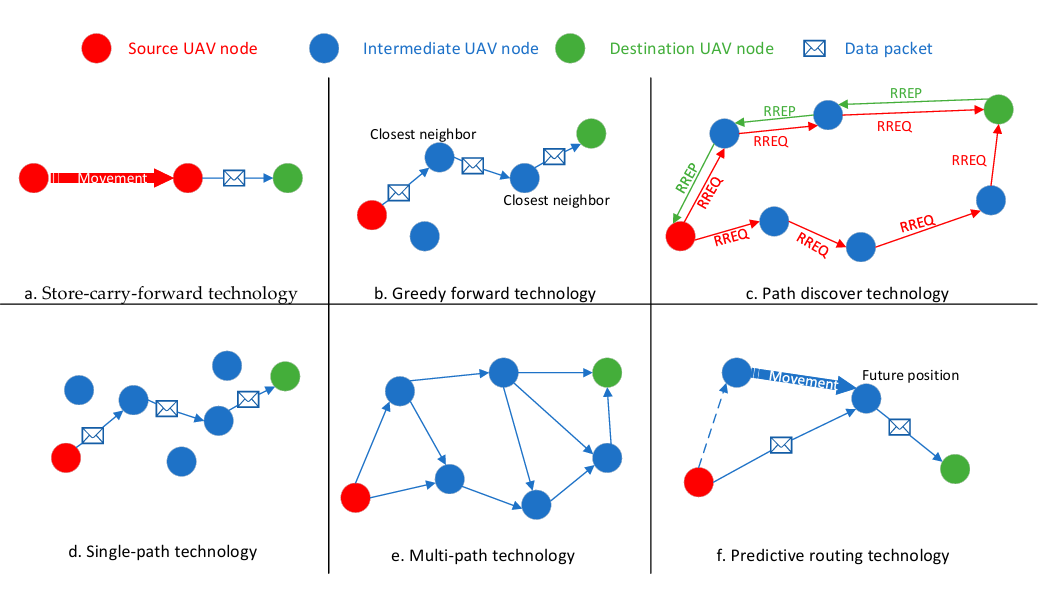
\includegraphics[width=0.9\textwidth]{Figures/Chapter1/Section6/1.png}
\caption{The rationales for common routing technologies of UAV ad hoc network.\cite{Chen2020}.}
\label{fig:The rationales for common routing technologies of UAV ad hoc network.}
\end{figure}



\begin{enumerate}
    \item \textbf{Store-carry-forward:} When no relay is available, the node stores and carries the data until it finds one. Suitable for intermittent networks but causes high delays.

    \item \textbf{Greedy forward:} Selects the neighbor closest to the destination as the next hop. Works well in dense UAV deployments but may fail if no closer neighbor exists requiring backup strategies.

    \item \textbf{Path discovery:} Uses flooding (RREQ) to find routes, improving path availability when location info is lost. However, it consumes significant bandwidth.

    \item \textbf{Single-path:} Sends data through one route, conserving bandwidth but lacking robustness no backup path if a failure occurs.

    \item \textbf{Multi-path:} Maintains several routes to improve reliability. If one path fails, others can take over. However, shared path failures can cause loops.

    \item \textbf{Predictive routing:} Estimates future positions based on current motion to choose the next hop. Ideal for high-mobility UAV swarms.
\end{enumerate}



%%%%%%%%%%%%%%%%%%%%%%%%%%%%%%%%%%%%%%%%%%%%%%%%%%%%%%%%%%%%%%%%%%%%%%

\subsection{The Classification of Routing Protocols}

Early research on UAV swarm communication focused on adapting traditional Ad hoc routing protocols. However, these proved largely unsuitable due to the unique characteristics of UAVs such as high mobility and varying mission requirements. As a result, researchers both enhanced existing protocols and developed new ones specifically for UAV swarms \cite{koubaa2017mavlink, Chen2020}. These routing protocols are now broadly categorized into three main types, each with several subtypes, as shown in ~\ref{fig:routing-protocols-classification}

\begin{figure}[ht]
\centering
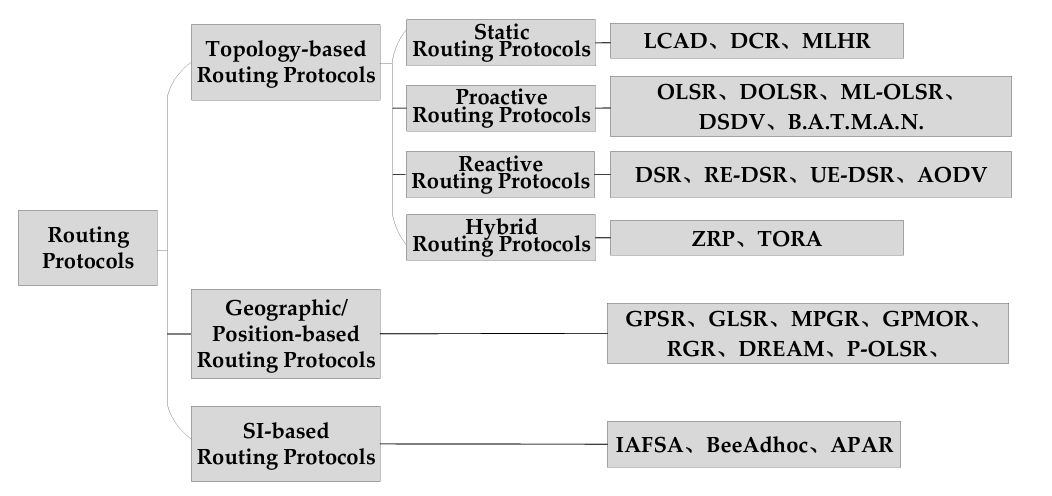
\includegraphics[width=0.7\textwidth]{Figures/Chapter1/Section6/2.png}
\caption{Classification of all routing protocols \cite{Chen2020}.}
\label{fig:routing-protocols-classification}
\end{figure}


%%%%%%%%%%%%%%%%%%%%%%%%%%%%%%%%%%%%%%%%%%%%%%%%%%%%%%%%%%%%%%%%%%%%%%

\subsection{Topology-Based Routing Protocols}

Topology-based routing protocols rely on IP addresses and known link information to forward packets efficiently. They are typically categorized into static, proactive, reactive, and hybrid protocols.

\subsubsection{Static Routing Protocols}


Static routing protocols use fixed routing tables and are suitable for stable topologies without task updates. Due to their lack of adaptability, their use in dynamic UAV swarms is limited. Notable examples include:

\begin{itemize}
    \item \textbf{Load Carry and Deliver (LCAD)}: Proposed by Le et al., LCAD uses a centralized system where a UAV carries and delivers data to its destination. It maximizes throughput and reduces hops but suffers from significant delays with increased communication distance.
    
    \item \textbf{Data Centric Routing (DCR)}: Designed for one-to-many transmission, DCR works well in “single-group swarm Ad hoc networks” with a gateway UAV distributing information. It’s ideal for small, planned UAV networks with minimal coordination between nodes.
    
    \item \textbf{Multilevel Hierarchical Routing (MLHR)}: Derived from vehicular networks, MLHR organizes UAVs into hierarchical layers, with gateway UAVs handling group-to-group communication ~\ref{fig:Multilevel Hierarchical Routing in a UAV swarm Ad hoc network}. It improves scalability and communication efficiency through geographic clustering.
\end{itemize}


\begin{figure}[ht]
\centering
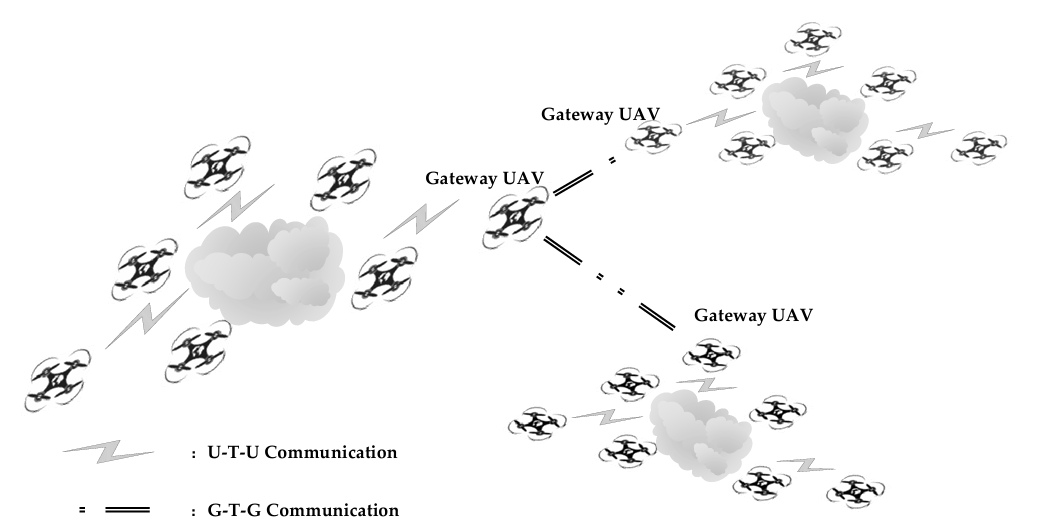
\includegraphics[width=0.7\textwidth]{Figures/Chapter1/Section6/3.png}
\caption{Multilevel Hierarchical Routing in a UAV swarm Ad hoc network}
\label{fig:Multilevel Hierarchical Routing in a UAV swarm Ad hoc network}
\end{figure}


\subsubsection{Proactive Routing Protocols}


Proactive routing protocols (PRPs) periodically update routing tables to reflect network topology, ensuring minimal route delays. While ideal for real-time applications, their frequent updates can be inefficient for fast-moving UAVs, especially in large-scale networks \cite{Chen2020}. Popular PRPs include Optimized Link State Routing (OLSR), Destination Sequenced Distance Vector (DSDV), and their variations.

\begin{itemize}
    \item \textbf{Optimized Link State Routing (OLSR)}: OLSR is a link-state protocol optimized for flat topologies~\cite{singh2015experimental}. It reduces overhead by selecting multiple point relays (MPR) for forwarding control packets, making it suitable for UAV ad hoc networks with dynamic topologies. Variants like Directional OLSR (DOLSR) and Mobility and Load-aware OLSR (ML-OLSR) further reduce latency and improve delivery rates.
    
    \item \textbf{Destination Sequenced Distance Vector (DSDV)}: In DSDV, routing tables are periodically updated, with either full or incremental dumps of routing information. While effective in stable networks, DSDV faces challenges in rapidly changing UAV networks, increasing bandwidth usage and overhead. It has been compared with other protocols in UAV networks.
    
    \item \textbf{B.A.T.M.A.N.}: This protocol proactively identifies the best next hop for each destination and maintains information about all nodes~\cite{sandhu2012performance}. B.A.T.M.A.N. performs similarly to OLSR in smaller networks but outperforms it in larger, bandwidth-constrained networks~\cite{sandhu2012performance}.
\end{itemize}



\subsubsection{Reactive Routing Protocols}

Reactive Routing Protocols (RRPs), also known as on-demand protocols, initiate route discovery only when needed, resulting in smaller routing information caches~\cite{Chen2020}. While RRPs generally have lower control overhead compared to PRPs, they suffer from high transmission delays due to the route discovery process. Popular RRPs include Dynamic Source Routing (DSR), Ad hoc On-Demand Distance Vector (AODV), and others.

\begin{itemize}
    \item \textbf{Dynamic Source Routing (DSR)}: DSR is widely used for ad hoc networks, requiring no specific infrastructure. It stores the complete list of routing nodes in each data packet, allowing the network to maintain performance despite topology changes. DSR has been adapted for UAV networks, with variants like Restrict DSR (RE-DSR) to limit hop counts and UAV Energy DSR (UE-DSR) for small UAVs in reconnaissance missions.
    
    \item \textbf{Ad hoc On-Demand Distance Vector (AODV)}: AODV reduces overhead by maintaining only destination addresses in routing tables. If a path is unavailable, the source node broadcasts Route Request (RREQ) to find a route. Once discovered, the Route Reply (RREP) is sent back to the source. Studies have explored AODV for UAV networks, with improvements aimed at minimizing hops and optimizing route reliability.
\end{itemize}


\subsubsection{Hybrid Routing Protocols}

To address the high overhead of control messages in PRPs and the delay in route discovery of RRPs, Hybrid Routing Protocols (HRPs) were introduced. HRPs divide large networks into zones, using PRP within zones and RRP between them ~\cite{Chen2020}. This strategy reduces routing overhead and delays but is challenged by the dynamic nature of UAV networks. Notable HRPs include Zone Routing Protocol (ZRP) and Temporarily Ordered Routing Algorithm (TORA).

\begin{itemize}
    \item \textbf{Zone Routing Protocol (ZRP)}: ZRP utilizes routing zones, applying PRP within zones and RRP for inter-zone communication. This reduces control packet overhead and delays compared to traditional PRPs and RRPs. ZRP's performance remains stable under high network load, but its fixed zone radius limits adaptability. Research focuses on improving ZRP with adaptive zones. Liu et al. proposed a clustering algorithm for UAV networks, while Zang et al. addressed cluster updates with mobility prediction.
    
    \item \textbf{Temporarily Ordered Routing Algorithm (TORA)}: TORA is a hybrid, distributed protocol designed for high adaptability. It minimizes control message spread by limiting updates to neighboring nodes and using longer routes to recover from link failures. TORA constructs a directed acyclic routing structure with "height" values to forward traffic effectively.
\end{itemize}

%%%%%%%%%%%%%%%%%%%%%%%%%%%%%%%%%%%%%%%%%%%%%%%%%%%%%%%%%%%%%%%%%%%%%%

\subsection{Geographic/Position-Based Routing Protocols}

Due to the high mobility in UAV ad hoc networks, maintaining routing tables becomes challenging, and traditional protocols introduce significant overhead. To address this, researchers have proposed position-based routing protocols that use location services, such as Reactive Location Services (RLS), Grid Location Services (GLS), and Hierarchical Location Services (HLS), which are well-suited for dynamic UAV networks ~\cite{Chen2020}.

\begin{itemize}
    \item \textbf{Greedy Perimeter Stateless Routing (GPSR)}: A position-based protocol that outperforms proactive and reactive protocols in UAV networks. It is especially effective in dense UAV deployments but requires further reliability improvements.
    
    \item \textbf{Geographic Load Share Routing (GLSR)}: An extension of GPSR, GLSR selects the next hop based on the "distance of advance" to improve path reliability.
    
    \item \textbf{Mobility Prediction-based Geographic Routing (MPGR)}: This protocol uses Gaussian motion prediction to evaluate node connectivity and select a reliable next hop.
    
    \item \textbf{Geographic Position Mobility Oriented Routing (GPMOR)}: Uses GPS and the Gaussian-Markov mobility model to predict UAV movement and improve routing decisions.
    
    \item \textbf{Reactive-Greedy-Reactive (RGR)}: Combines AODV with Greedy Geographic Forwarding (GGF), switching between AODV and GGF based on connectivity. It improves packet delivery but can suffer from packet loss if position information isn't updated.
    
    \item \textbf{DREAM}: A location-based protocol using a location table to store node coordinates, consuming less bandwidth but being more complex than flooding strategies.
    
    \item \textbf{Prediction-OLSR}: A protocol that uses GPS to assist routing decisions, adjusting based on node speed and expected transmission count.
\end{itemize}

%%%%%%%%%%%%%%%%%%%%%%%%%%%%%%%%%%%%%%%%%%%%%%%%%%%%%%%%%%%%%%%%%%%%%%

\subsection{Swarm Intelligence-Based Routing Protocols}

Swarm intelligence (SI) is a multi-agent system inspired by the behavior of animals like fish, birds, and insects. It is applied to mobile robots and enhances collaborative task optimization. In UAV swarm systems, SI is used to improve routing protocols \cite{zungerua2012classical}.

For example, the \textbf{Improved Artificial Fish-Swarm Algorithm (IAFSA)} adjusts group topology to address communication range expansion and information leakage, ensuring secure communication in large swarms. Other SI-based routing protocols include the \textbf{Bee colony algorithm-based Ad hoc network (BeeAdhoc)} and the \textbf{Ant Colony Optimization-based Polymorphism-Aware Routing (APAR)}.


%%%%%%%%%%%%%%%%%%%%%%%%%%%%%%%%%%%%%%%%%%%%%%%%%%%%%%%%%%%%%%%%%%%%%%
\subsection{Discussion}

Static routing protocols are unsuitable for UAV swarm Ad hoc networks due to fixed routing tables and limited scalability. Proactive protocols incur high overhead for maintaining up-to-date tables and react slowly to topology changes. Reactive protocols suffer from high latency in route discovery. Source routing does not scale well due to large network overhead and header size. Hybrid protocols combine proactive and reactive methods to address these issues, but dynamic nodes and link behaviors in UAV networks complicate information maintenance. Topology-based protocols are not ideal for highly dynamic networks with many nodes. Geographic/position-based routing protocols, by incorporating node location data, excel in handling high mobility and frequent topology changes in UAV networks.



%%%%%%%%%%%%%%%%%%%%%%%%%%%%%%%%%%%%%%%%%%%%%%%%%%%%%%%%%%%%%%%%%%%%%%
%%%%%%%%%%%%%%%%%%%%%%%%%%%%%%%%%%%%%%%%%%%%%%%%%%%%%%%%%%%%%%%%%%%%%%
%%%%%%%%%%%%%%%%%%%%%%%%%%%%%%%%%%%%%%%%%%%%%%%%%%%%%%%%%%%%%%%%%%%%%%



\section{Conclusion}


This chapter has presented the main elements that define the structure and functionality of UAV systems. It has covered the various UAV types including multirotors, fixed-wing, and hybrid designs, as well as performance-related characteristics such as weight, endurance, and propulsion methods. These classification frameworks help in selecting the right UAVs for different use cases and also support a better understanding of how these systems connect and communicate. As UAV technologies continue to advance and expand into more complex applications, it becomes increasingly important to understand their technical foundations and communication protocols. The content of this chapter lays the groundwork for further study into communication systems, interoperability issues, and the integration of UAVs within intelligent and collaborative environments.